% ==========================================
% BAB II STUDI LITERATUR (REVISED - FINAL)
% ==========================================
\chapter{STUDI LITERATUR}
\label{chap:studi-literatur}

Bab ini menyajikan tinjauan komprehensif terhadap literatur yang relevan dengan pengembangan sistem rangkuman otomatis berbasis \textit{AI} untuk mereduksi \textit{information overload} dalam komunitas finansial. Tinjauan mencakup enam domain utama: (1) \textit{Information Overload} dan \textit{Cognitive Load Theory} sebagai landasan teoretis, (2) Fondasi arsitektur \textit{Transformer}, BERT, dan evolusi menuju \textit{Large Language Models}, (3) \textit{Text Summarization} dengan model bahasa skala besar, (4) Analisis teks finansial mencakup sentimen, emosi, dan ekstraksi entitas, (5) Infrastruktur sistem yang mengintegrasikan platform, arsitektur \textit{real-time}, \textit{topic modeling}, dan \textit{pipeline} pemrosesan, dan (6) Kesenjangan penelitian. Setiap domain memberikan landasan teoretis dan metodologis untuk pengembangan sistem rangkuman otomatis.

% ==========================================
\section{\textit{Information Overload} dan \textit{Cognitive Load Theory}}
\label{sec:information-overload}

\textit{Information overload} merupakan fenomena yang terjadi ketika individu dihadapkan pada volume informasi yang melampaui kapasitas kognitif mereka untuk memproses secara efektif \autocite{eppler2004}. Dalam konteks komunitas online, khususnya platform media sosial seperti Telegram, masalah ini menjadi semakin akut karena tingginya laju produksi dan distribusi informasi. Bagian ini mengulas teori-teori fundamental yang menjelaskan bagaimana \textit{information overload} memengaruhi pengambilan keputusan, serta mengidentifikasi strategi mitigasi melalui sistem otomatis berbasis \textit{AI}.

\subsection{Konsep dan Dampak \textit{Information Overload}}

Penelitian seminal oleh \textcite{eppler2004} menyediakan landasan teoretis komprehensif tentang konsep \textit{information overload}. Berdasarkan tinjauan literatur dari berbagai disiplin ilmu termasuk \textit{Organization Science}, Akuntansi, Pemasaran, dan Sistem Informasi Manajemen, mereka mendefinisikan \textit{information overload} sebagai kondisi yang terjadi ketika kualitas pengambilan keputusan menurun karena kuantitas informasi yang tersedia melampaui kapasitas pemrosesan individu. Studi tersebut mengidentifikasi hubungan inverted U-curve antara kuantitas informasi dan kualitas keputusan, yang menunjukkan bahwa setelah mencapai titik optimal, penambahan informasi justru menurunkan performa kognitif.

\begin{figure}[H]
  \centering
  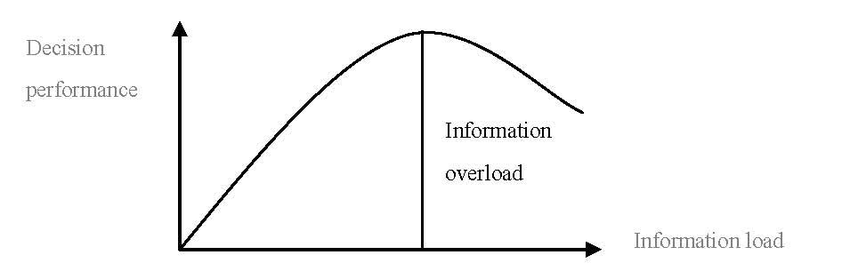
\includegraphics[width=0.7\textwidth]{image/information-overload-curve.png}
  \caption{Hubungan \textit{inverted U-curve} antara kuantitas informasi dan kualitas pengambilan keputusan, menunjukkan titik optimal dan zona \textit{overload} (diadaptasi dari \textcite{eppler2004})}
  \label{fig:info-overload}
\end{figure}

\textcite{shahrzadi2024} memperkuat pemahaman ini melalui \textit{scoping review} terbaru yang menganalisis penyebab, konsekuensi, dan strategi penanganan \textit{information overload}. Penelitian mereka mengidentifikasi tiga kategori penyebab utama: (1) faktor personal seperti keterbatasan kapasitas kognitif dan kurangnya keterampilan manajemen informasi, (2) karakteristik informasi seperti ambiguitas, kompleksitas, dan ketidakpastian, dan (3) parameter teknologi informasi termasuk intensitas notifikasi dan desain antarmuka. Dampak yang diidentifikasi mencakup penurunan produktivitas, kualitas keputusan yang buruk, stres, dan kelelahan kognitif. Strategi mitigasi berbasis teknologi yang diidentifikasi mencakup penggunaan \textit{filtering tools} dan sistem otomatis untuk mereduksi volume informasi.

\subsection{Landasan Teori: \textit{Cognitive Load Theory}}

\textit{Cognitive Load Theory} (CLT), yang dikembangkan oleh \textcite{sweller1988}, memberikan kerangka teoretis untuk memahami keterbatasan kapasitas memori kerja manusia dalam pemrosesan informasi. Teori ini mengidentifikasi tiga jenis beban kognitif: (1) \textit{intrinsic load}, yang inheren dengan kompleksitas materi yang dipelajari, (2) \textit{extraneous load}, yang dihasilkan oleh cara informasi disajikan, dan (3) \textit{germane load}, yang berkontribusi pada pembentukan skema dan otomatisasi. Dalam konteks komunitas online, pengguna menghadapi \textit{intrinsic load} yang tinggi karena kompleksitas informasi finansial, sementara desain antarmuka platform media sosial sering kali meningkatkan \textit{extraneous load} melalui notifikasi, pesan yang tidak terstruktur, dan kurangnya organisasi informasi.

\begin{figure}[H]
  \centering
  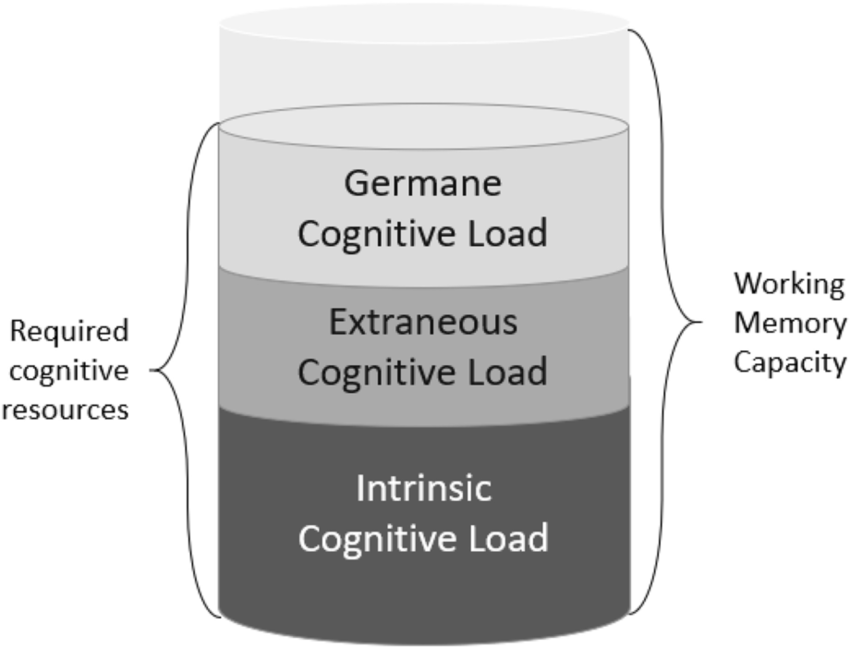
\includegraphics[width=0.75\textwidth]{image/cognitive-load-theory.png}
  \caption{Tiga jenis beban kognitif dalam \textit{Cognitive Load Theory}: \textit{intrinsic}, \textit{extraneous}, dan \textit{germane load} (diadaptasi dari \textcite{sweller1988})}
  \label{fig:cognitive-load}
\end{figure}

\textcite{skulmowski2022} mengembangkan pemahaman CLT dengan mengadaptasinya untuk lingkungan digital dan pembelajaran daring. Penelitian mereka mengusulkan perspektif baru tentang \textit{extraneous cognitive load} yang mempertimbangkan karakteristik unik media digital, seperti konten yang kaya secara perseptual, distraksi visual, dan desain antarmuka yang kompleks. Mereka berargumen bahwa media digital menciptakan bentuk \textit{extraneous load} yang berbeda dari media tradisional, terutama melalui elemen-elemen yang tidak relevan dengan tujuan pembelajaran atau pemrosesan informasi inti.

Penelitian empiris oleh \textcite{sidnammauch2024} menerapkan CLT secara khusus pada konteks distraksi media sosial melalui studi dengan 1.026 partisipan. Mereka mengintegrasikan \textit{load theory of attention} dengan kerangka \textit{uses and gratifications} untuk menjelaskan bagaimana media sosial mobile menciptakan distraksi melalui sumber daya kognitif yang terbatas. Studi mereka mendemonstrasikan bahwa individu dengan kapasitas memori kerja yang lebih rendah lebih rentan terhadap distraksi media sosial, dan bahwa \textit{affordances} teknologi seperti notifikasi \textit{push} dan aksesibilitas konstan memperburuk masalah ini.

\subsection{Ekonomi Perhatian di Media Sosial}

\textcite{heitmayer2025} memberikan perspektif teoretis terbaru dengan mengusulkan bahwa perhatian (\textit{attention}) berfungsi sebagai mata uang simbolis universal di media sosial. Penelitian ini memperkenalkan model \textit{dual-stream} yang membedakan antara perhatian yang "mengalir" (\textit{flow attention}) dan perhatian yang "mengeras" (\textit{calcified attention}). \textit{Flow attention} mengacu pada alokasi perhatian yang dinamis dan sementara terhadap konten yang terus berubah, sementara \textit{calcified attention} merujuk pada investasi perhatian jangka panjang yang termanifestasi dalam bentuk \textit{followers}, \textit{likes}, atau keanggotaan komunitas. Kelangkaan perhatian (\textit{attention scarcity}) yang diidentifikasi menjadi masalah sentral yang harus diatasi oleh sistem rangkuman otomatis.

Analisis empiris oleh \textcite{nematzadeh2019} tentang \textit{information overload} dalam komunikasi grup menggunakan data dari platform Twitch menunjukkan bagaimana peningkatan volume pesan dalam grup dapat menyebabkan transisi dari percakapan yang koheren menjadi "kakofoni" sehingga informasi bermakna tenggelam dalam kebisingan. Mereka mengidentifikasi bahwa ketika laju pesan melebihi ambang batas tertentu, kualitas percakapan menurun drastis, partisipasi menjadi tidak merata, dan informasi penting hilang.


% ==========================================
\section{Fondasi Arsitektur: \textit{Transformer} dan BERT}
\label{sec:transformer-bert}

Arsitektur fundamental yang mendasari perkembangan NLP modern mencakup \textit{Transformer} dan \textit{Bidirectional Encoder Representations from Transformers} (BERT). Bagian ini mengulas inovasi arsitektural yang telah merevolusi pemrosesan bahasa alami dan menjadi fondasi bagi hampir semua model bahasa kontemporer.

\subsection{Arsitektur \textit{Transformer}}

\textcite{vaswani2017} memperkenalkan arsitektur \textit{Transformer} yang menggantikan arsitektur rekuren tradisional (\textit{RNN}, \textit{LSTM}) dengan mekanisme \textit{self-attention} yang dapat memproses seluruh urutan input secara paralel. Inovasi kunci dari \textit{Transformer} adalah kemampuannya untuk menangkap dependensi jarak jauh dalam teks tanpa keterbatasan memori yang dialami oleh arsitektur rekuren. Mekanisme \textit{multi-head attention} memungkinkan model untuk menghadiri berbagai aspek representasional input secara simultan, sementara \textit{positional encoding} mempertahankan informasi tentang urutan kata. Arsitektur \textit{encoder-decoder} yang diusulkan terdiri dari tumpukan lapisan \textit{transformer} yang masing-masing mengandung sub-lapisan \textit{multi-head self-attention} dan \textit{feed-forward neural network}.

\begin{figure}[H]
  \centering
  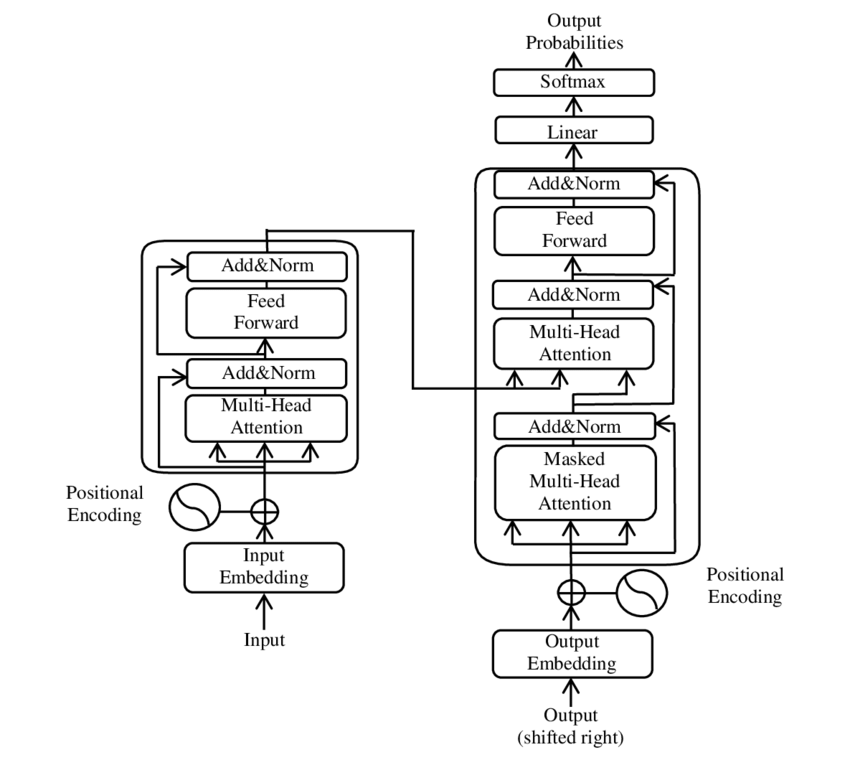
\includegraphics[width=0.65\textwidth]{image/transformer-architecture.png}
  \caption{Arsitektur Transformer dengan mekanisme \textit{multi-head attention} dan struktur \textit{encoder-decoder} (diadaptasi dari \textcite{vaswani2017})}
  \label{fig:transformer-arch}
\end{figure}

\subsection{BERT dan Representasi \textit{Bidirectional}}

\textcite{devlin2019} mengembangkan konsep \textit{Transformer} lebih lanjut dengan memperkenalkan BERT, model bahasa yang dilatih secara \textit{bidirectional} menggunakan arsitektur \textit{Transformer encoder}. Berbeda dengan model bahasa \textit{unidirectional} sebelumnya yang hanya memproses teks dari kiri ke kanan atau kanan ke kiri, BERT dilatih menggunakan dua tugas pra-latih: \textit{Masked Language Modeling} (MLM), yaitu sebagian token input di-\textit{mask} dan model harus memprediksinya berdasarkan konteks bidirectional, dan \textit{Next Sentence Prediction} (NSP). Model memprediksi apakah dua kalimat berurutan dalam teks original. Pendekatan \textit{pre-training} dan \textit{fine-tuning} yang diusulkan memungkinkan BERT untuk mencapai performa \textit{state-of-the-art} pada sebelas tugas NLP yang beragam. Representasi kontekstual bidirectional yang dihasilkan BERT menangkap nuansa semantik yang tidak dapat ditangkap oleh model unidirectional atau representasi statis seperti Word2Vec.

\begin{figure}[H]
  \centering
  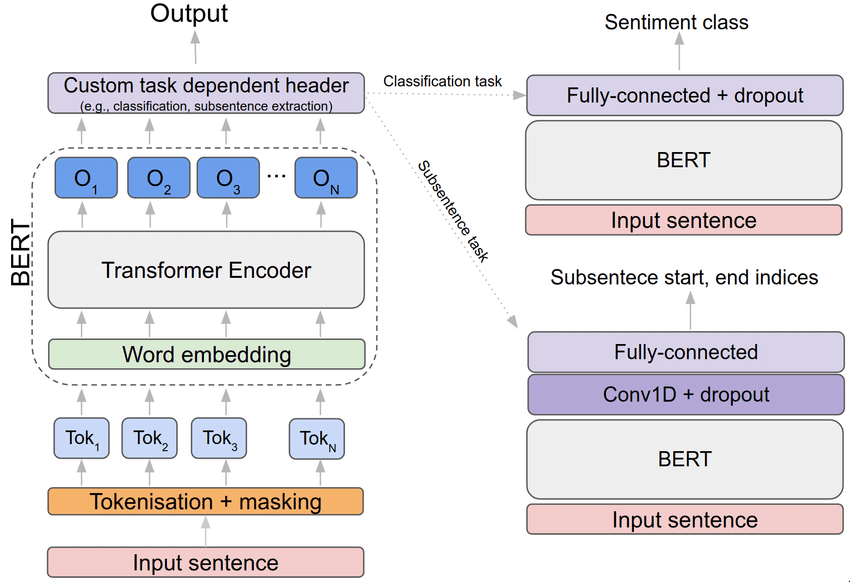
\includegraphics[width=0.85\textwidth]{image/bert-architecture-diagram.png}
  \caption{Arsitektur BERT menunjukkan mekanisme \textit{bidirectional self-attention} dan proses \textit{pre-training} dengan \textit{Masked Language Modeling} (diadaptasi dari \textcite{devlin2019})}
  \label{fig:bert-architecture}
\end{figure}

Kontribusi BERT terhadap NLP tidak hanya terletak pada performa superiornya pada berbagai \textit{benchmark}, tetapi juga pada paradigma \textit{transfer learning} yang efektif: model bahasa umum yang besar dilatih pada korpus teks masif, kemudian di-\textit{fine-tune} untuk tugas spesifik dengan data berlabel yang relatif terbatas.

\subsection{IndoBERT untuk Bahasa Indonesia}

\textcite{wilie2020} memperkenalkan \textit{IndoNLU}, benchmark komprehensif untuk evaluasi pemahaman bahasa Indonesia yang mencakup dua belas tugas termasuk analisis sentimen. Dataset mereka dilatih pada \textit{Indo4B}, korpus bahasa Indonesia dengan empat miliar kata, dan menyediakan model IndoBERT yang mengungguli \textit{multilingual BERT} (mBERT) pada berbagai tugas. Penelitian ini mendemonstrasikan bahwa model bahasa monolingual yang dilatih khusus pada korpus bahasa Indonesia menghasilkan performa superior dibandingkan model multilingual untuk tugas-tugas NLP Indonesia.

Penelitian oleh \textcite{koto2020} memperkuat temuan ini dengan memperkenalkan \textit{IndoLEM}, benchmark dataset dan model IndoBERT untuk NLP Indonesia. Mereka mendemonstrasikan bahwa \textit{pre-training} pada korpus bahasa Indonesia yang besar (220 juta kata) menghasilkan representasi bahasa yang lebih baik untuk tugas-tugas \textit{downstream}, yang mencapai F1-score 84,13\% untuk analisis sentimen.

\subsection{Evolusi Menuju \textit{Large Language Models}}

Perkembangan arsitektur \textit{Transformer} dan BERT menjadi fondasi bagi evolusi model bahasa dengan skala parameter yang jauh lebih besar. Evolusi ini mengikuti dua jalur paralel yang berbeda: jalur \textit{encoder} (BERT dan variannya) dan jalur \textit{decoder-only} (GPT dan variannya), dengan munculnya model \textit{open-source} skala besar seperti LLaMA yang memberikan alternatif terhadap model proprietary.

\textcite{brown2020} memperkenalkan GPT-3, model bahasa autoregresif dengan 175 miliar parameter, 10 kali lebih besar dari model \textit{non-sparse} sebelumnya. GPT-3 mendemonstrasikan kemampuan \textit{few-shot learning}, yakni model dapat melakukan tugas baru hanya dengan beberapa contoh tanpa \textit{fine-tuning}, sebuah kemampuan emergen yang muncul dari skala model yang sangat besar. Penelitian ini menetapkan paradigma baru dalam NLP yaitu \textit{scaling up} ukuran model secara dramatis meningkatkan kemampuan \textit{task-agnostic} dan \textit{in-context learning}.

\textcite{touvron2023} memperkenalkan LLaMA, koleksi model bahasa fondasi dengan range 7B hingga 65B parameter yang dilatih menggunakan dataset publik secara eksklusif. Penelitian ini mendemonstrasikan bahwa model \textit{state-of-the-art} dapat dilatih tanpa bergantung pada dataset proprietary yang tidak dapat diakses. LLaMA-13B mengungguli GPT-3 (175B) pada sebagian besar \textit{benchmark}, sementara LLaMA-65B kompetitif dengan model terbaik seperti Chinchilla-70B dan PaLM-540B. Karakteristik \textit{open-source} dari LLaMA telah memfasilitasi pengembangan ekosistem model turunan dan aplikasi spesifik domain.

Evolusi menuju LLMs ini didorong oleh \textit{scaling laws} yang menghubungkan peningkatan jumlah parameter dan data dengan peningkatan performa, serta munculnya kemampuan emergen seperti \textit{few-shot learning} dan \textit{in-context learning} yang tidak dimiliki model skala kecil. Model-model ini menjadi fondasi bagi berbagai aplikasi NLP kontemporer, termasuk peringkasan teks, \textit{question answering}, dan generasi konten.


% ==========================================
\section{\textit{Text Summarization} dengan \textit{Large Language Models}}
\label{sec:text-summarization}

Peringkasan teks otomatis telah mengalami evolusi signifikan dengan munculnya model bahasa berbasis \textit{transformer} dan \textit{large language models} (LLMs). Bagian ini mengulas perkembangan metodologi peringkasan teks dari pendekatan berbasis ekstraksi hingga generasi abstraktif dengan LLMs, dengan fokus khusus pada tantangan peringkasan multi-dokumen, percakapan, dan media sosial.

\subsection{Peringkasan Berbasis \textit{Transformer}}

\textcite{liu2019bertsum} memperkenalkan pendekatan \textit{BERTSum} yang memanfaatkan representasi BERT untuk peringkasan ekstraktif dan abstraktif. Penelitian mereka mendemonstrasikan bahwa model \textit{encoder} tingkat dokumen yang dibangun di atas BERT dengan lapisan \textit{Transformer} antar-kalimat dapat menghasilkan rangkuman berkualitas tinggi. Pendekatan dua tahap \textit{fine-tuning} yang mereka usulkan, yaitu model pertama-tama di-\textit{fine-tune} untuk tugas ekstraksi kalimat sebelum dilatih untuk generasi abstraktif, menetapkan metodologi dasar yang diadopsi oleh banyak penelitian berikutnya.

Pemahaman tentang \textit{trade-off} antara peringkasan ekstraktif dan abstraktif diperluas oleh penelitian \textcite{pilault2020}, yang membandingkan kedua pendekatan menggunakan model \textit{transformer} pada dokumen panjang. Evaluasi manusia mereka mengungkapkan temuan penting: sementara pendekatan abstraktif berbasis \textit{transformer} unggul dalam koherensi dan kelancaran, metode ekstraktif cenderung mencetak lebih tinggi dalam hal informativeness. Temuan ini menginformasikan desain sistem hibrida yang mengkombinasikan ekstraksi topik dengan generasi naratif.

\begin{figure}[H]
  \centering
  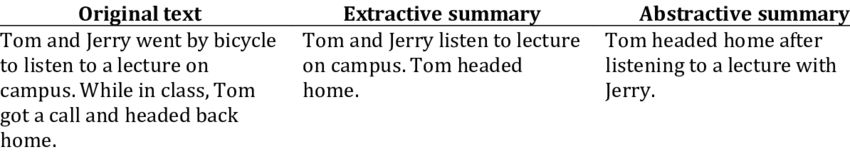
\includegraphics[width=0.8\textwidth]{image/extractive-vs-abstractive.png}
  \caption{Perbandingan pendekatan peringkasan ekstraktif (memilih kalimat penting) dan abstraktif (menghasilkan teks baru) menunjukkan \textit{trade-off} antara \textit{informativeness} dan koherensi}
  \label{fig:extract-abstract}
\end{figure}

\subsection{Peringkasan Multi-Dokumen dan Sintesis Informasi}

\textcite{deyoung2024} mengajukan pertanyaan fundamental: apakah model peringkasan multi-dokumen modern benar-benar dapat mensintesis informasi, atau hanya melakukan agregasi sederhana? Melalui evaluasi terhadap berbagai model dari \textit{fine-tuned transformers} hingga GPT-4, mereka menemukan bahwa sebagian besar model mengalami kesulitan dalam mensintesis informasi yang bertentangan atau berbeda perspektif, dan sangat sensitif terhadap urutan input dokumen. Temuan kritis ini memiliki implikasi langsung bagi desain sistem: sistem harus dirancang dengan mekanisme eksplisit untuk menangani informasi yang mungkin bertentangan, dan tidak boleh bergantung semata-mata pada kemampuan sintesis implisit LLM.

\textcite{ravaut2024} menyediakan wawasan penting tentang bagaimana LLMs memanfaatkan konteks panjang dalam peringkasan. Penelitian mereka mengungkapkan masalah \textit{position bias}, yaitu LLMs cenderung memberikan bobot yang tidak merata terhadap informasi berdasarkan posisinya dalam konteks. Mereka mengevaluasi enam LLMs berbeda pada sepuluh dataset dengan lima metrik evaluasi, menemukan bahwa model cenderung memberikan perhatian berlebihan pada informasi di awal dan akhir konteks, sementara mengabaikan informasi di tengah. Desain sistem harus mempertimbangkan strategi mitigasi \textit{position bias}, seperti pengelompokan pesan berdasarkan topik sebelum peringkasan atau penggunaan rangkuman inkremental.

\subsection{Peringkasan Percakapan dan Dialog}

\textcite{gliwa2019} memperkenalkan \textit{SAMSum Corpus}, dataset dialog yang dianotasi secara manual untuk peringkasan abstraktif, yang menetapkan bahwa peringkasan percakapan memiliki tantangan unik dibandingkan dengan peringkasan artikel berita. Dialog dan percakapan grup memiliki struktur yang lebih kompleks dengan pergantian pembicara, konteks implisit, referensi anaforik, dan topik yang bercabang.

\textcite{tian2024} mengembangkan metodologi peringkasan dialog lebih lanjut dengan mengusulkan pendekatan \textit{Mixture of Experts} (MoE) berbasis LLM. Penelitian mereka memperkenalkan mekanisme \textit{role-oriented routing} yang memilih model atau strategi peringkasan yang sesuai berdasarkan karakteristik informasi percakapan yang berbeda. Pendekatan ini relevan dengan konteks komunitas finansial berjenjang, yakni pesan dari berbagai peran mungkin memerlukan perlakuan berbeda dalam proses peringkasan.

\textcite{chen2021} mengusulkan pendekatan yang sadar struktur (\textit{structure-aware}) untuk peringkasan percakapan abstraktif. Penelitian mereka memodelkan relasi wacana dan \textit{action triples} ("siapa-melakukan-apa") menggunakan graf terstruktur untuk menangkap karakteristik kompleks interaksi manusia-manusia di media sosial. Mereka mengimplementasikan mekanisme \textit{decoding} multi-granularitas yang dapat menghasilkan rangkuman pada tingkat abstraksi berbeda.

\textcite{fabbri2021} memperkenalkan \textit{ConvoSumm}, benchmark peringkasan percakapan yang mencakup empat dataset dari berbagai bentuk percakapan online. Penelitian mereka menggunakan \textit{framework} \textit{issues-viewpoints-assertions} yang menginkorporasikan \textit{argument mining} melalui konstruksi graf untuk memodelkan struktur percakapan. Pendekatan ini mengakui bahwa percakapan online sering kali melibatkan pertukaran pandangan yang kompleks dengan argumen pendukung.

\textcite{sotudeh2021} memperkenalkan dataset TLDR9+ dengan lebih dari 9 juta \textit{instance} pelatihan dari Reddit untuk peringkasan ekstrim (rangkuman satu kalimat). Mereka mendemonstrasikan bahwa peringkasan ekstrim, yang menghasilkan rangkuman sangat singkat dengan tingkat kompresi dan abstraksi tinggi, dapat efektif untuk konten media sosial yang cenderung verbose.

\subsection{Memori Jangka Panjang dalam Sistem Dialog}

\textcite{wang2023recursive} mengusulkan metode peringkasan rekursif untuk memungkinkan LLMs mempertahankan konteks percakapan yang panjang. Pendekatan mereka melibatkan pembuatan rangkuman hierarkis dari konteks dialog yang kemudian digunakan untuk menjaga konsistensi dalam percakapan yang berkepanjangan. Konsep ini paralel dengan desain sistem rangkuman per jam; dalam desain ini, setiap rangkuman per jam dapat dipandang sebagai pembentukan "memori jangka panjang" bagi komunitas.

\subsection{Metrik Evaluasi untuk Peringkasan}

\textcite{zhang2020bertscore} memperkenalkan \textit{BERTScore}, metrik evaluasi yang menggunakan \textit{contextual embeddings} dari BERT untuk menghitung kesamaan antara rangkuman yang dihasilkan dan rangkuman referensi, mengatasi keterbatasan metrik berbasis \textit{n-gram} seperti ROUGE yang hanya menghitung kecocokan kata eksak. \textit{BERTScore} mendemonstrasikan korelasi yang lebih baik dengan penilaian manusia karena dapat mengenali parafrase dan kesamaan semantik.

\textcite{shen2023} memberikan peringatan penting tentang penggunaan LLMs sebagai evaluator otomatis untuk peringkasan abstraktif. Melalui analisis ekstensif terhadap ChatGPT dan GPT-4 sebagai evaluator, mereka menemukan masalah signifikan dalam stabilitas, reliabilitas, dan ketergantungan pada dimensi evaluasi tertentu. Temuan mereka menunjukkan bahwa evaluasi otomatis berbasis LLM tidak dapat sepenuhnya menggantikan evaluasi manusia, terutama untuk aspek kualitatif seperti koherensi naratif dan relevansi kontekstual.

\subsection{Tantangan Inferensi LLM dalam Sistem \textit{Real-Time}}

Bottleneck arsitektural yang paling signifikan dalam sistem rangkuman otomatis berbasis LLM adalah latensi inferensi model bahasa besar. Tidak seperti komponen NLP tradisional seperti tokenisasi atau \textit{named entity recognition} yang dapat dieksekusi dalam milidetik, generasi teks dengan LLM skala besar (puluhan hingga ratusan miliar parameter) dapat memerlukan waktu detik hingga menit untuk satu panggilan inferensi.

Penelitian terkini menunjukkan bahwa kecepatan inferensi LLM sangat dipengaruhi oleh tiga faktor utama: (1) ukuran model (jumlah parameter), (2) panjang konteks input, dan (3) infrastruktur komputasi yang digunakan (CPU, GPU, atau akselerator khusus seperti TPU). Model yang lebih besar seperti Llama 3.1 70B, meskipun memberikan kualitas output superior, memerlukan sumber daya komputasi yang substansial. Solusi arsitektural termasuk penggunaan akselerator khusus seperti \textit{Language Processing Unit} (LPU) yang dirancang untuk inferensi LLM dengan kecepatan ekstrem, serta strategi optimasi seperti \textit{quantization} dan \textit{batching}.

\subsection{Standar Latensi dan Keterbacaan untuk Sistem Rangkuman}

Penetapan target latensi sistem memerlukan pemahaman tentang karakteristik performa infrastruktur LLM modern. Penelitian empiris oleh \textcite{groq2024} mendemonstrasikan bahwa Groq LPU mencapai throughput 284 token per detik untuk Llama 3.1 70B dalam mode standar, dengan optimasi \textit{speculative decoding} meningkatkan performa hingga 1.660 token per detik, diverifikasi secara independen oleh Artificial Analysis. Untuk tugas peringkasan tipikal dengan output 2.000 token, waktu inferensi berkisar antara 7 hingga 20 detik tergantung pada konfigurasi infrastruktur dan beban sistem. Infrastruktur \textit{enterprise-grade} seperti NVIDIA HGX H200 dengan 8× Tensor Core GPUs mencapai 268 token per detik per pengguna dengan Medusa \textit{speculative decoding} \autocite{nvidia2024}, menghasilkan waktu total sekitar 15 detik untuk rangkuman 2.000 token termasuk \textit{overhead} pemrosesan. Studi independen oleh \textcite{dilmegani2024} pada lima LLM terkemuka untuk tugas peringkasan 500-token menunjukkan waktu penyelesaian berkisar 11-38 detik, mengonfirmasi bahwa target latensi 5 menit (300 detik) menyediakan margin keamanan 15-40 kali lipat untuk mengakomodasi variabilitas jaringan, antrian, dan overhead pemrosesan dalam skenario produksi.

Dari perspektif konsumsi informasi, kecepatan membaca manusia rata-rata adalah 238 kata per menit untuk teks non-fiksi berdasarkan meta-analisis 190 studi yang melibatkan 18.573 partisipan dewasa \autocite{brysbaert2019}. Rentang tipikal untuk pembaca dewasa adalah 175-300 kata per menit. Durasi membaca 3 menit memungkinkan konsumsi 525-750 kata, yang mengakomodasi spektrum kemampuan pembaca sambil tetap berada dalam batasan kapasitas memori kerja manusia. Teori beban kognitif (\textit{Cognitive Load Theory}) menetapkan bahwa memori kerja manusia dapat memproses 7 ± 2 item secara simultan dengan durasi sekitar 20 detik tanpa pengulangan \autocite{cowan2001}. Rangkuman dengan panjang 600-750 kata yang dapat dibaca dalam 3 menit memastikan bahwa konten dapat diproses tanpa saturasi memori kerja, memungkinkan bandwidth kognitif yang cukup untuk pemahaman, integrasi dengan pengetahuan sebelumnya, dan retensi informasi.


% ==========================================
\section{Analisis Teks Finansial: Sentimen, Emosi, dan Entitas}
\label{sec:financial-text-analysis}

Analisis teks finansial merupakan komponen esensial dalam memahami dinamika diskusi di media sosial. Bagian ini membahas ekstraksi sinyal-sinyal spesifik dari teks: sentimen dan emosi yang mencerminkan psikologi pasar, serta entitas finansial yang menjadi objek diskusi. Ketiga komponen ini—sentimen, emosi, dan ekstraksi entitas—bersifat komplementer dalam sistem rangkuman.

\subsection{Model Bahasa untuk Analisis Sentimen Indonesia}

\textcite{nugroho2021} menerapkan \textit{fine-tuning} BERT untuk analisis sentimen pada ulasan aplikasi mobile berbahasa Indonesia, konteks yang memiliki kesamaan dengan teks media sosial karena sifatnya yang informal dan sering mengandung bahasa gaul atau singkatan. Penelitian mereka membandingkan model multibahasa dengan model khusus Indonesia, mendemonstrasikan keunggulan \textit{transfer learning} untuk bahasa Indonesia dengan data berlabel terbatas.

\subsection{Analisis Sentimen Domain Finansial}

\textcite{araci2019} memperkenalkan \textit{FinBERT}, model BERT pertama yang dilatih khusus pada korpus finansial untuk analisis sentimen. Model ini mencapai peningkatan akurasi 15\% dibandingkan BERT umum pada dataset \textit{Financial PhraseBank} dan FiQA. Penelitian ini mendemonstrasikan pentingnya \textit{domain-specific pre-training} untuk teks finansial, yang memiliki karakteristik linguistik unik termasuk terminologi khusus dan nuansa sentimen yang berbeda dari domain umum.

\textcite{si2014} mengeksplorasi pemanfaatan sentimen media sosial untuk prediksi pergerakan saham dengan mengintegrasikan analisis sentimen Twitter dengan struktur relasi sosial. Penelitian mereka mendemonstrasikan bahwa menggabungkan sentimen dengan informasi jaringan sosial secara signifikan meningkatkan akurasi prediksi. Temuan kunci mereka adalah bahwa tidak semua opini memiliki bobot yang sama; pendapat dari individu yang lebih berpengaruh atau kredibel dalam jaringan sosial harus diberi bobot lebih tinggi.

\subsection{Klasifikasi Emosi vs Sentimen untuk Investor Ritel}

Penelitian perilaku keuangan menunjukkan bahwa keputusan investasi ritel sangat dipengaruhi oleh emosi, terutama ketakutan (\textit{fear}) dan keserakahan (\textit{greed}). Berbeda dengan analis profesional yang dilatih untuk membuat keputusan berdasarkan analisis rasional, investor ritel sering kali membuat keputusan yang didorong oleh reaksi emosional terhadap pergerakan pasar atau diskusi komunitas.

Model klasifikasi emosi dapat mendeteksi spektrum emosi yang lebih nuansa, termasuk ketakutan, kegembiraan, kemarahan, dan kesedihan. Emosi-emosi ini memberikan sinyal yang lebih kaya tentang psikologi pasar dibandingkan dengan sentimen biner. Misalnya, ekspresi ketakutan tinggi dalam diskusi komunitas dapat mengindikasikan potensi \textit{panic selling}, sementara kegembiraan berlebihan dapat menandakan \textit{euphoria} yang sering kali mendahului koreksi pasar.

Konteks diskusi informal di platform seperti Telegram lebih cenderung mengekspresikan emosi autentik dibandingkan dengan laporan finansial formal atau analisis profesional. Klasifikasi emosi dapat menangkap sinyal-sinyal psikologis ini yang hilang dalam analisis sentimen tradisional.

\begin{figure}[H]
  \centering
  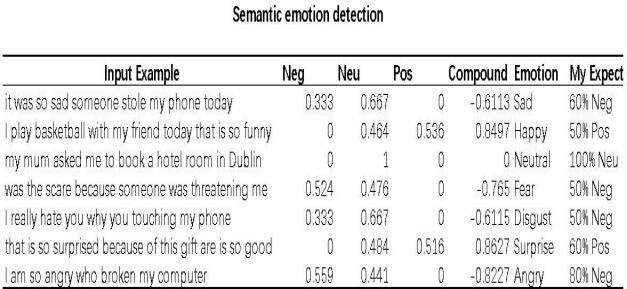
\includegraphics[width=0.75\textwidth]{image/sentiment-analysis-example.jpg}
  \caption{Contoh klasifikasi emosi pada teks menggunakan model \textit{semantic emotion detection}, menunjukkan deteksi berbagai emosi seperti \textit{sad}, \textit{happy}, \textit{fear}, \textit{disgust}, \textit{surprise}, dan \textit{angry} beserta skor probabilitasnya}
  \label{fig:sentiment-example}
\end{figure}

\subsection{Pemanfaatan Sinyal Komunitas dalam Peringkasan}

\textcite{kano2018} mengusulkan metodologi inovatif untuk memanfaatkan sinyal popularitas dalam media sosial (seperti \textit{votes}, \textit{shares}, \textit{bookmarks}) sebagai label jarak jauh (\textit{distant labels}) untuk peringkasan ekstraktif percakapan online. Penelitian mereka mendemonstrasikan bahwa metrik keterlibatan komunitas dapat berfungsi sebagai indikator kualitas dan relevansi konten. Pendekatan ini relevan dengan konteks komunitas finansial berjenjang, yakni struktur hierarkis dan peran pengguna dapat dimanfaatkan sebagai sinyal implisit tentang pentingnya informasi. Sistem \textit{weighted sentiment} dapat memberikan bobot lebih tinggi pada pesan dari sumber yang lebih kredibel atau berpengaruh dalam komunitas.

\subsection{\textit{Named Entity Recognition} untuk Teks Finansial Indonesia}

\textit{Named Entity Recognition} (NER) merupakan tugas fundamental dalam NLP yang bertujuan mengidentifikasi dan mengklasifikasikan entitas bernama dalam teks, seperti nama orang, organisasi, lokasi, dan dalam konteks finansial, nama perusahaan dan kode saham (ticker).

\textcite{khairunnisa2020} mengidentifikasi masalah kritis dalam dataset NER Indonesia yang ada: inkonsistensi anotasi yang dapat menurunkan performa model. Mereka menyediakan dataset yang dianotasi ulang dengan standar yang lebih konsisten dan mengevaluasi berbagai pendekatan \textit{deep learning}. Penelitian mereka menekankan pentingnya kualitas data pelatihan dan konsistensi skema anotasi untuk mencapai performa NER yang optimal.

\begin{figure}[H]
  \centering
  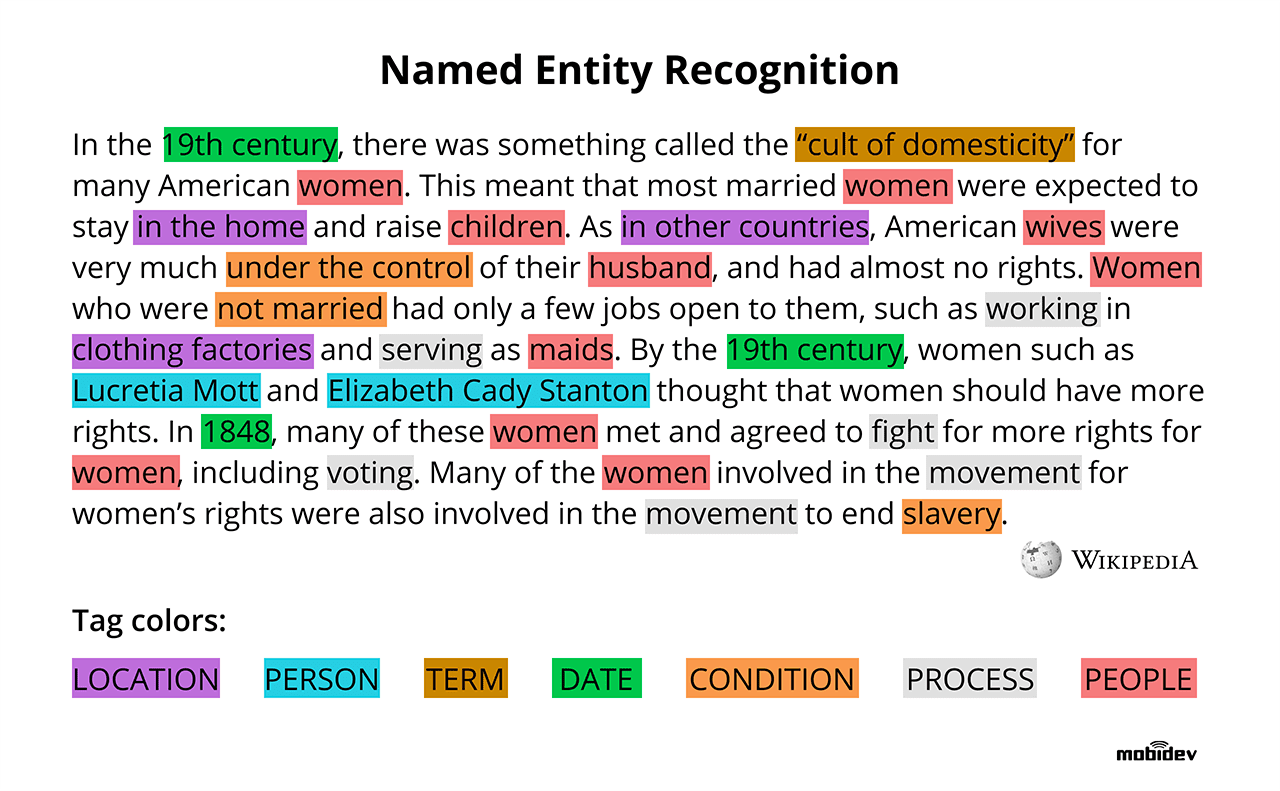
\includegraphics[width=0.85\textwidth]{image/ner-example.png}
  \caption{Contoh \textit{Named Entity Recognition} pada teks, menunjukkan identifikasi berbagai jenis entitas seperti nama orang (\textit{PERSON}), lokasi (\textit{LOCATION}), tanggal (\textit{DATE}), dan istilah khusus (\textit{TERM}) yang diberikan label dan warna berbeda}
  \label{fig:ner-example}
\end{figure}

\textcite{zhang2022finbert} mengembangkan \textit{FinBERT-MRC}, pendekatan NER finansial yang merumuskan tugas ekstraksi entitas sebagai masalah \textit{machine reading comprehension}. Model mereka mencapai F1-score 92,78\% dan 96,80\% pada dataset finansial. Penelitian ini mendemonstrasikan bahwa NER domain finansial memiliki tantangan unik karena variasi semantik dan leksikal yang spesifik.

\textcite{shah2023} menyediakan \textit{FiNER-ORD}, dataset NER finansial \textit{open research} pertama dengan kualitas tinggi. Penelitian mereka menekankan bahwa entitas finansial sering kali memiliki representasi multipel (misalnya, "Apple Inc.", "Apple", "AAPL") yang harus dikenali sebagai entitas yang sama.

\subsection{Standar Akurasi NER untuk Domain Finansial Indonesia}

Penetapan target akurasi untuk NER domain finansial memerlukan pemahaman tentang baseline performa untuk bahasa Indonesia dan standar industri untuk aplikasi finansial. Penelitian oleh \textcite{dave2024} pada ekstraksi entitas finansial personal Indonesia menggunakan IndoBERT-BiGRU-CRF mencapai F1-score 73\% untuk 15 kategori entitas finansial (tipe pengeluaran, jumlah pendapatan, tipe aset). Penelitian ini menetapkan baseline performa untuk NER finansial Indonesia dengan dataset terbatas (1.138 kalimat), mendemonstrasikan bahwa akurasi 70-75\% dapat dicapai dengan model monolingual Indonesia yang dioptimalkan untuk domain finansial.

Untuk NER finansial dalam bahasa Inggris, analisis industri oleh \textcite{phoenix2024} menunjukkan bahwa sistem domain-spesifik mencapai akurasi 92-95\%, jauh melampaui sistem \textit{general-purpose} yang hanya mencapai 75-80\%. Perbedaan signifikan ini menunjukkan bahwa model yang dilatih pada dataset finansial dengan kosakata domain-spesifik memberikan peningkatan akurasi 25\% dibandingkan sistem generik. Sekitar 85\% kesalahan klasifikasi berasal dari kurangnya kesadaran kontekstual, mengindikasikan pentingnya mekanisme \textit{context-aware} dalam NER finansial. Untuk NER Indonesia umum (nama orang, lokasi, organisasi), penelitian oleh \textcite{khairunnisa2020} menunjukkan bahwa model BiLSTM-CRF baseline mencapai F1-score 90,85\%, sementara IndoBERT-BiLSTM-CRF mencapai 94,90\%. Penurunan signifikan ke 73\% untuk entitas finansial mendemonstrasikan tantangan tambahan dalam ekstraksi domain finansial, menjadikan target 80\% sebagai threshold realistis antara baseline Indonesia (73\%) dan standar sistem matang (92-95\%).


% ==========================================
\section{Infrastruktur Sistem: Platform, Arsitektur, dan \textit{Pipeline}}
\label{sec:system-infrastructure}

Implementasi sistem rangkuman otomatis untuk komunitas yang aktif memerlukan pemahaman mendalam tentang karakteristik platform, arsitektur pemrosesan yang dapat menangani aliran data \textit{real-time}, komponen analisis yang dapat beroperasi secara asinkron, dan integrasi \textit{pipeline} yang kohesif.

\subsection{Karakteristik Platform Telegram}

\textcite{nobari2017} menyediakan analisis pionir tentang struktur dan aspek topikal Telegram menggunakan data yang di-\textit{crawl} dari kanal publik. Penelitian mereka mengeksplorasi pola jaringan dan arsitektur Telegram sebagai platform \textit{messaging} hibrida yang menggabungkan fitur komunikasi pribadi dan publik. Mereka mengidentifikasi bahwa Telegram memiliki karakteristik unik: kombinasi antara privasi komunikasi dengan kemampuan penyebaran informasi massal melalui kanal dan grup besar.

\textcite{hashemi2019} mengembangkan metodologi untuk mengukur kualitas grup Telegram melalui analisis perilaku pengguna. Mereka mengusulkan fitur-fitur pengukuran kualitas yang membedakan grup berkualitas tinggi dari grup berkualitas rendah berdasarkan pola aktivitas pengguna, konsistensi partisipasi, dan struktur komunikasi. Penelitian mereka menunjukkan bahwa grup berkualitas tinggi cenderung memiliki partisipasi yang lebih seimbang, topik diskusi yang lebih fokus, dan tingkat spam yang lebih rendah.

\textcite{lamorgia2024} menyediakan dataset Telegram terbesar dengan 120.979 kanal dan lebih dari 400 juta pesan, bersama dengan infrastruktur untuk pengumpulan dan analisis data skala besar. Kontribusi mereka mendemonstrasikan bahwa Telegram telah berkembang menjadi ekosistem informasi yang kompleks dengan dinamika komunitas yang beragam.

\textcite{perlo2025} menyediakan analisis per-topik pertama dari grup Telegram, mengeksplorasi 51 juta pesan dari 669 grup di berbagai topik termasuk Cryptocurrency. Temuan kunci mereka adalah bahwa grup dengan topik berbeda menunjukkan pola komunikasi yang sangat berbeda dalam hal volume pesan, distribusi waktu aktivitas, dan tipe konten yang dibagikan. Khususnya untuk kategori Cryptocurrency, mereka menemukan tingkat aktivitas yang sangat tinggi dengan puncak aktivitas yang berkorelasi dengan jam perdagangan pasar.

\subsection{Arsitektur Sistem \textit{Real-time} dan \textit{Event-Driven}}

\textcite{hamidi2021} mengusulkan arsitektur \textit{pipeline} NLP yang dinamis dan terdistribusi untuk pemrosesan \textit{stream} teks \textit{real-time}. Penelitian mereka menggunakan Apache Storm dan Apache Kafka untuk menerapkan tugas-tugas NLP pada aliran data tekstual. Arsitektur mereka mendemonstrasikan bagaimana komponen NLP yang berbeda dapat dikomposisikan dalam \textit{pipeline} yang dapat di-\textit{scale} secara horizontal.

\textcite{isah2019} menyediakan survei komprehensif tentang \textit{framework} pemrosesan \textit{stream} data terdistribusi. Penelitian mereka membandingkan model pemrosesan, karakteristik operasional, dan pola arsitektural dari berbagai \textit{framework}. Untuk konteks dengan volume pesan yang tinggi namun tidak ekstrem, mereka mengidentifikasi bahwa pendekatan \textit{micro-batch processing} atau arsitektur berbasis \textit{event} yang lebih sederhana dapat memberikan keseimbangan optimal antara latensi, throughput, dan kompleksitas implementasi.

\textcite{rubert2023} menyediakan bukti empiris tentang dampak \textit{event-driven architecture} (EDA) terhadap performa melalui studi eksploratif. Penelitian mereka mendemonstrasikan bahwa EDA dapat memberikan keunggulan signifikan dalam \textit{scalability} dan responsivitas, terutama untuk sistem yang menangani beban kerja yang bervariasi dan tidak dapat diprediksi.

Pendekatan \textit{micro-batching} sering kali lebih praktis untuk banyak aplikasi NLP. Konsep rangkuman periodik dapat dipandang sebagai bentuk \textit{macro-batching}, yaitu pesan dikumpulkan selama periode waktu tertentu sebelum diproses sebagai satu \textit{batch}. Pendekatan ini memberikan beberapa keuntungan: memungkinkan agregasi konteks yang lebih kaya untuk tugas-tugas seperti \textit{topic modeling}, mengurangi beban komputasi, dan sesuai dengan ritme natural konsumsi informasi pengguna.

\subsection{Komponen Analisis Asinkron: \textit{Topic Modeling} dengan BERTopic}

\textcite{grootendorst2022} memperkenalkan BERTopic, metodologi \textit{topic modeling} neural yang menggabungkan model bahasa berbasis \textit{transformer}, \textit{document embeddings}, \textit{clustering} dengan HDBSCAN, dan prosedur \textit{class-based TF-IDF} (c-TF-IDF). Arsitektur BERTopic mengatasi keterbatasan pendekatan tradisional seperti \textit{Latent Dirichlet Allocation} (LDA) dengan memanfaatkan representasi semantik kontekstual. Metodologi ini sangat sesuai untuk teks media sosial yang pendek dan informal.

\begin{figure}[H]
  \centering
  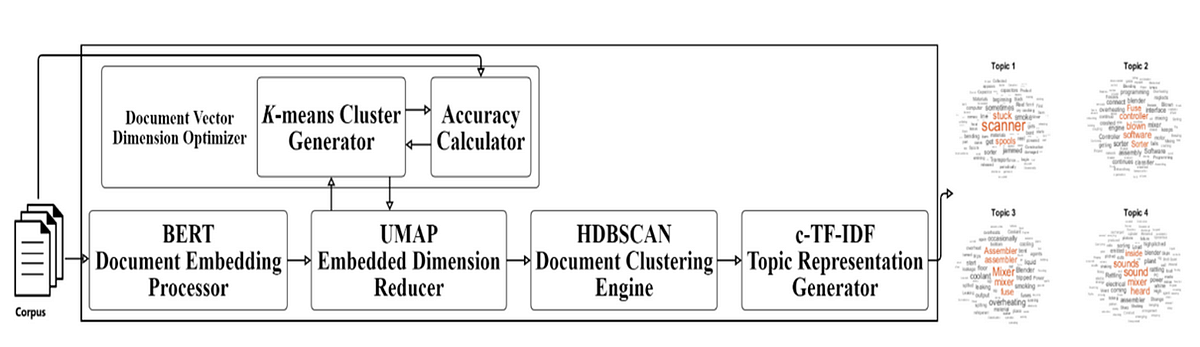
\includegraphics[width=0.85\textwidth]{image/bertopic-workflow.png}
  \caption{Alur kerja BERTopic menunjukkan tahapan dari \textit{document embeddings}, dimensionality reduction dengan UMAP, \textit{clustering} dengan HDBSCAN, hingga ekstraksi representasi topik dengan c-TF-IDF (diadaptasi dari \textcite{grootendorst2022})}
  \label{fig:bertopic-workflow}
\end{figure}

Keunggulan BERTopic untuk teks media sosial divalidasi secara empiris oleh \textcite{egger2022}, yang membandingkan BERTopic dengan LDA, NMF, dan Top2Vec pada dataset 31.800 \textit{tweet}. Evaluasi mereka mendemonstrasikan superioritas BERTopic untuk teks pendek dan tidak terstruktur, khususnya dalam hal koherensi topik dan interpretabilitas.

Interpretasi skor koherensi topik memerlukan pemahaman tentang skala dan ambang batas kualitas yang dapat diterima. Penelitian oleh \textcite{roeder2015} menetapkan bahwa metrik C\_v (koherensi berbasis konteks) menghasilkan korelasi terkuat dengan penilaian manusia tentang interpretabilitas topik, dengan rentang nilai 0 hingga 1. Berdasarkan meta-analisis praktisi NLP dan studi empiris yang dikompilasi oleh \textcite{hoyle2021}, konsensus muncul bahwa skor C\_v antara 0,4-0,5 merepresentasikan kualitas topik yang dapat diterima (\textit{borderline acceptable}), skor 0,5-0,6 menunjukkan kualitas baik, dan skor di atas 0,6 mengindikasikan kualitas sangat baik dengan interpretabilitas tinggi. Untuk aplikasi produksi yang melayani pengguna non-teknis, target minimum 0,5 memastikan bahwa topik yang dihasilkan dapat dipahami tanpa keahlian domain mendalam, kriteria yang esensial untuk sistem rangkuman komunitas finansial ritel.

\textcite{angelov2024} mengembangkan metodologi \textit{topic modeling} lebih lanjut dengan memperkenalkan \textit{Contextual-Top2Vec}. Penelitian mereka mengusulkan penggunaan \textit{BERTScore} untuk mengevaluasi koherensi dan informativeness topik, mengatasi keterbatasan metrik evaluasi tradisional.

\subsection{Integrasi \textit{Pipeline} dan Tantangannya}

Integrasi \textit{pipeline} NLP multi-komponen menghadapi beberapa tantangan teknis. Pertama, \textbf{manajemen dependensi antar komponen}: beberapa komponen mungkin memerlukan output dari komponen lain sebagai input. Kedua, \textbf{penanganan kegagalan parsial}: jika satu komponen gagal, sistem harus dapat melanjutkan pemrosesan. Ketiga, \textbf{konsistensi temporal}: semua komponen harus memproses data dari periode waktu yang sama untuk memastikan rangkuman yang koheren.

Dalam arsitektur \textit{event-driven}, setiap komponen NLP dapat dipandang sebagai \textit{event handler} yang independen. Pendekatan ini memungkinkan setiap komponen untuk beroperasi secara paralel ketika memungkinkan, sambil mempertahankan dependensi yang diperlukan.

Tantangan khusus yang diidentifikasi adalah \textbf{koordinasi antara pemrosesan \textit{batch} periodik dan arsitektur \textit{event-driven}}. Solusi yang umum digunakan adalah menggunakan \textit{temporal windowing}: pesan dikumpulkan dalam jendela waktu, dan pada akhir jendela, \textit{event} pemicu dihasilkan untuk memulai \textit{pipeline} pemrosesan.

Integrasi dengan API inferensi LLM menambahkan dimensi lain: \textbf{penanganan layanan eksternal asinkron}. Panggilan API bersifat asinkron dan dapat mengalami latensi variabel. Sistem harus dirancang dengan mekanisme \textit{timeout}, \textit{retry logic}, dan fallback untuk menangani kegagalan sementara atau latensi tinggi.

\textbf{Observabilitas dan monitoring \textit{pipeline}} menjadi kritis dalam sistem produksi. Setiap komponen harus menghasilkan metrik dan log yang memungkinkan operator untuk memahami performa sistem, mengidentifikasi bottleneck, dan mendiagnosis kegagalan.


% ==========================================
\section{Penelitian Basis Utama}
\label{sec:research-foundation}

Berdasarkan tinjauan literatur yang komprehensif, penelitian ini dibangun di atas tiga fondasi metodologis utama yang dipilih karena relevansi langsung dengan karakteristik komunitas Telegram finansial Indonesia yang hierarkis dan memiliki volume pesan tinggi. Bagian ini mengidentifikasi penelitian-penelitian basis yang menjadi referensi utama beserta justifikasi pemilihannya.

\subsection{BERTopic untuk \textit{Topic Modeling} Teks Media Sosial}

Penelitian \textcite{grootendorst2022} tentang BERTopic dipilih sebagai fondasi untuk komponen identifikasi topik diskusi. BERTopic dirancang khusus untuk mengatasi tantangan \textit{topic modeling} pada teks pendek dan informal seperti pesan media sosial. Metodologi ini mengintegrasikan model bahasa berbasis \textit{transformer} untuk \textit{contextual embeddings}, algoritma HDBSCAN untuk \textit{clustering} adaptif, dan prosedur \textit{class-based TF-IDF} untuk ekstraksi representasi topik.

Pemilihan BERTopic dijustifikasi oleh tiga alasan utama. Pertama, superioritas untuk teks pendek yang divalidasi secara empiris oleh \textcite{egger2022} yang membandingkan BERTopic dengan LDA, NMF, dan Top2Vec pada dataset 31.800 \textit{tweet}, mendemonstrasikan keunggulan BERTopic dalam hal koherensi topik dan interpretabilitas. Kedua, kemampuan menghasilkan topik yang interpretatif sangat penting untuk sistem rangkuman yang harus dipahami oleh investor ritel tanpa keahlian teknis NLP. Ketiga, \textit{clustering} berbasis kepadatan dengan HDBSCAN sesuai dengan karakteristik diskusi Telegram yang memiliki topik dengan densitas berbeda-beda.

\subsection{\textit{Weighted Influence System} dari Analisis Sentimen Media Sosial}

Penelitian \textcite{si2014} tentang pemanfaatan sentimen media sosial untuk prediksi pergerakan saham menyediakan fondasi teoretis untuk sistem \textit{weighted influence}. Temuan kunci mereka bahwa "tidak semua opini memiliki bobot yang sama" dan bahwa pendapat dari individu yang lebih berpengaruh atau kredibel dalam jaringan sosial harus diberi bobot lebih tinggi menjadi prinsip desain fundamental sistem rangkuman.

Penelitian \textcite{si2014} menggunakan metrik jaringan sosial seperti \textit{centrality} dan jumlah \textit{followers} untuk menentukan bobot pengaruh. Prinsip bahwa kontribusi dari aktor yang lebih sentral dalam jaringan harus memiliki dampak lebih besar dalam agregasi sentimen diadaptasi untuk konteks komunitas finansial hierarkis. Sistem rangkuman yang diusulkan mengeksploitasi struktur hierarkis eksplisit komunitas Telegram Michael Yeoh untuk memberikan bobot berbeda pada kontribusi dari Michael Yeoh (pemimpin komunitas), administrator, VIP members, dan regular members.

\subsection{Peringkasan Percakapan \textit{Structure-Aware}}

Penelitian \textcite{chen2021} tentang peringkasan percakapan abstraktif yang \textit{structure-aware} menyediakan kerangka metodologis untuk menangani kompleksitas diskusi multi-pihak dalam media sosial. Pendekatan mereka yang memodelkan relasi wacana dan \textit{action triples} ("siapa-melakukan-apa") menggunakan graf terstruktur relevan dengan tantangan meringkas diskusi finansial yang sering kali melibatkan pertukaran argumen, rekomendasi, dan analisis yang kompleks.

Prinsip \textit{structure-awareness} dan konsep \textit{multi-granular decoding} yang dapat menghasilkan rangkuman pada tingkat abstraksi berbeda menginspirasi desain format rangkuman \textit{mixed} yang menggabungkan \textit{bullet points} untuk informasi terstruktur (saham, sinyal, metrik) dengan paragraf naratif untuk konteks dan analisis. Penelitian ini juga menghadapi tantangan tambahan yaitu sintesis informasi dari empat grup dengan karakteristik komunikasi berbeda, yang memerlukan adaptasi pendekatan \textit{structure-aware} untuk konteks multi-grup.

\subsection{Justifikasi Pemilihan dan Integrasi}

Ketiga penelitian ini dipilih karena komplementaritas metodologis mereka dalam menangani aspek-aspek kritis sistem rangkuman untuk komunitas finansial. BERTopic menangani identifikasi topik dari teks informal, \textit{weighted influence system} menangani prioritisasi berdasarkan kredibilitas sumber, dan pendekatan \textit{structure-aware} menangani generasi rangkuman yang koheren dan informatif.

Integrasi ketiga fondasi ini, serta detail implementasi teknis, arsitektur sistem, dan adaptasi spesifik untuk konteks komunitas Telegram finansial Indonesia akan dijelaskan secara komprehensif dalam Bab \ref{chap:desain-konsep-solusi} tentang Desain Konsep Solusi.


% ==========================================
\section{Konteks Penelitian: Komunitas Telegram Michael Yeoh}
\label{sec:konteks-penelitian}

Penelitian ini dilakukan dalam konteks komunitas investasi saham Indonesia Michael Yeoh di platform Telegram, yang merupakan salah satu komunitas finansial ritel terbesar di Indonesia dengan lebih dari 47.000 anggota. Komunitas ini menyediakan wadah untuk edukasi pasar, analisis saham, dan diskusi strategi investasi yang terfokus pada pasar modal Indonesia.

Komunitas Michael Yeoh mengadopsi struktur hierarkis empat tingkat yang dirancang untuk menyediakan nilai berbeda pada setiap level keanggotaan. Struktur ini terdiri dari: (1) \textbf{MY Cuap Cuap} dengan sekitar 20.500 anggota yang berfungsi sebagai kanal edukasi umum dengan mode \textit{broadcast}, (2) \textbf{MY Swing Plan} dengan sekitar 20.500 anggota yang mendistribusikan sinyal \textit{trading} terstruktur, (3) \textbf{MY Advanced Group} dengan sekitar 4.300 anggota premium yang memiliki akses ke diskusi interaktif dua arah dengan volume sekitar 200 pesan per jam selama jam perdagangan, dan (4) \textbf{MY PIRANHA} dengan sekitar 2.000 anggota ultra-premium yang mengalami volume diskusi tertinggi (lebih dari 200 pesan per jam) dengan karakteristik percakapan yang kasual namun mendalam secara konten.

Struktur hierarkis ini menciptakan ekosistem informasi yang kompleks dengan aliran informasi vertikal dari puncak hierarki (Michael Yeoh dan administrator) ke berbagai level anggota. Namun, struktur ini juga menghasilkan dua tantangan signifikan yang menjadi fokus penelitian ini. Pertama, \textbf{\textit{information overload}} yang parah di grup premium (Advanced dan PIRANHA) dengan volume pesan yang mencapai 200+ pesan per jam, jauh melampaui kapasitas kognitif anggota untuk memproses informasi secara efektif. Kedua, \textbf{fragmentasi informasi} lintas empat grup yang memerlukan anggota untuk melakukan sintesis manual antara analisis makro (Cuap Cuap), sinyal konkret (Swing Plan), diskusi implementasi (Advanced), dan debat strategi (PIRANHA).

Karakteristik unik komunitas ini—volume pesan ekstrim, struktur hierarkis eksplisit, konten domain finansial Indonesia, dan penggunaan Bahasa Indonesia informal—menjadikannya kasus yang ideal untuk pengembangan dan evaluasi sistem rangkuman otomatis berbasis \textit{AI} yang dioptimalkan untuk konteks lokal. Sistem yang dikembangkan dalam penelitian ini dirancang untuk mereduksi beban informasi melalui rangkuman periodik yang mensintesis intelijen lintas-grup, dengan memanfaatkan literatur tentang \textit{information overload}, \textit{cognitive load theory}, NLP finansial, dan infrastruktur sistem \textit{real-time} yang telah diulas dalam bab ini.

\subsection{Model Konseptual Sistem Komunikasi Komunitas}

Gambar \ref{fig:current-system} mengilustrasikan arsitektur sistem komunikasi komunitas saat ini beserta aliran informasi antar komponen. Model konseptual ini menunjukkan empat grup dengan karakteristik berbeda yang membentuk ekosistem informasi hierarkis.

\begin{figure}[H]
  \centering
  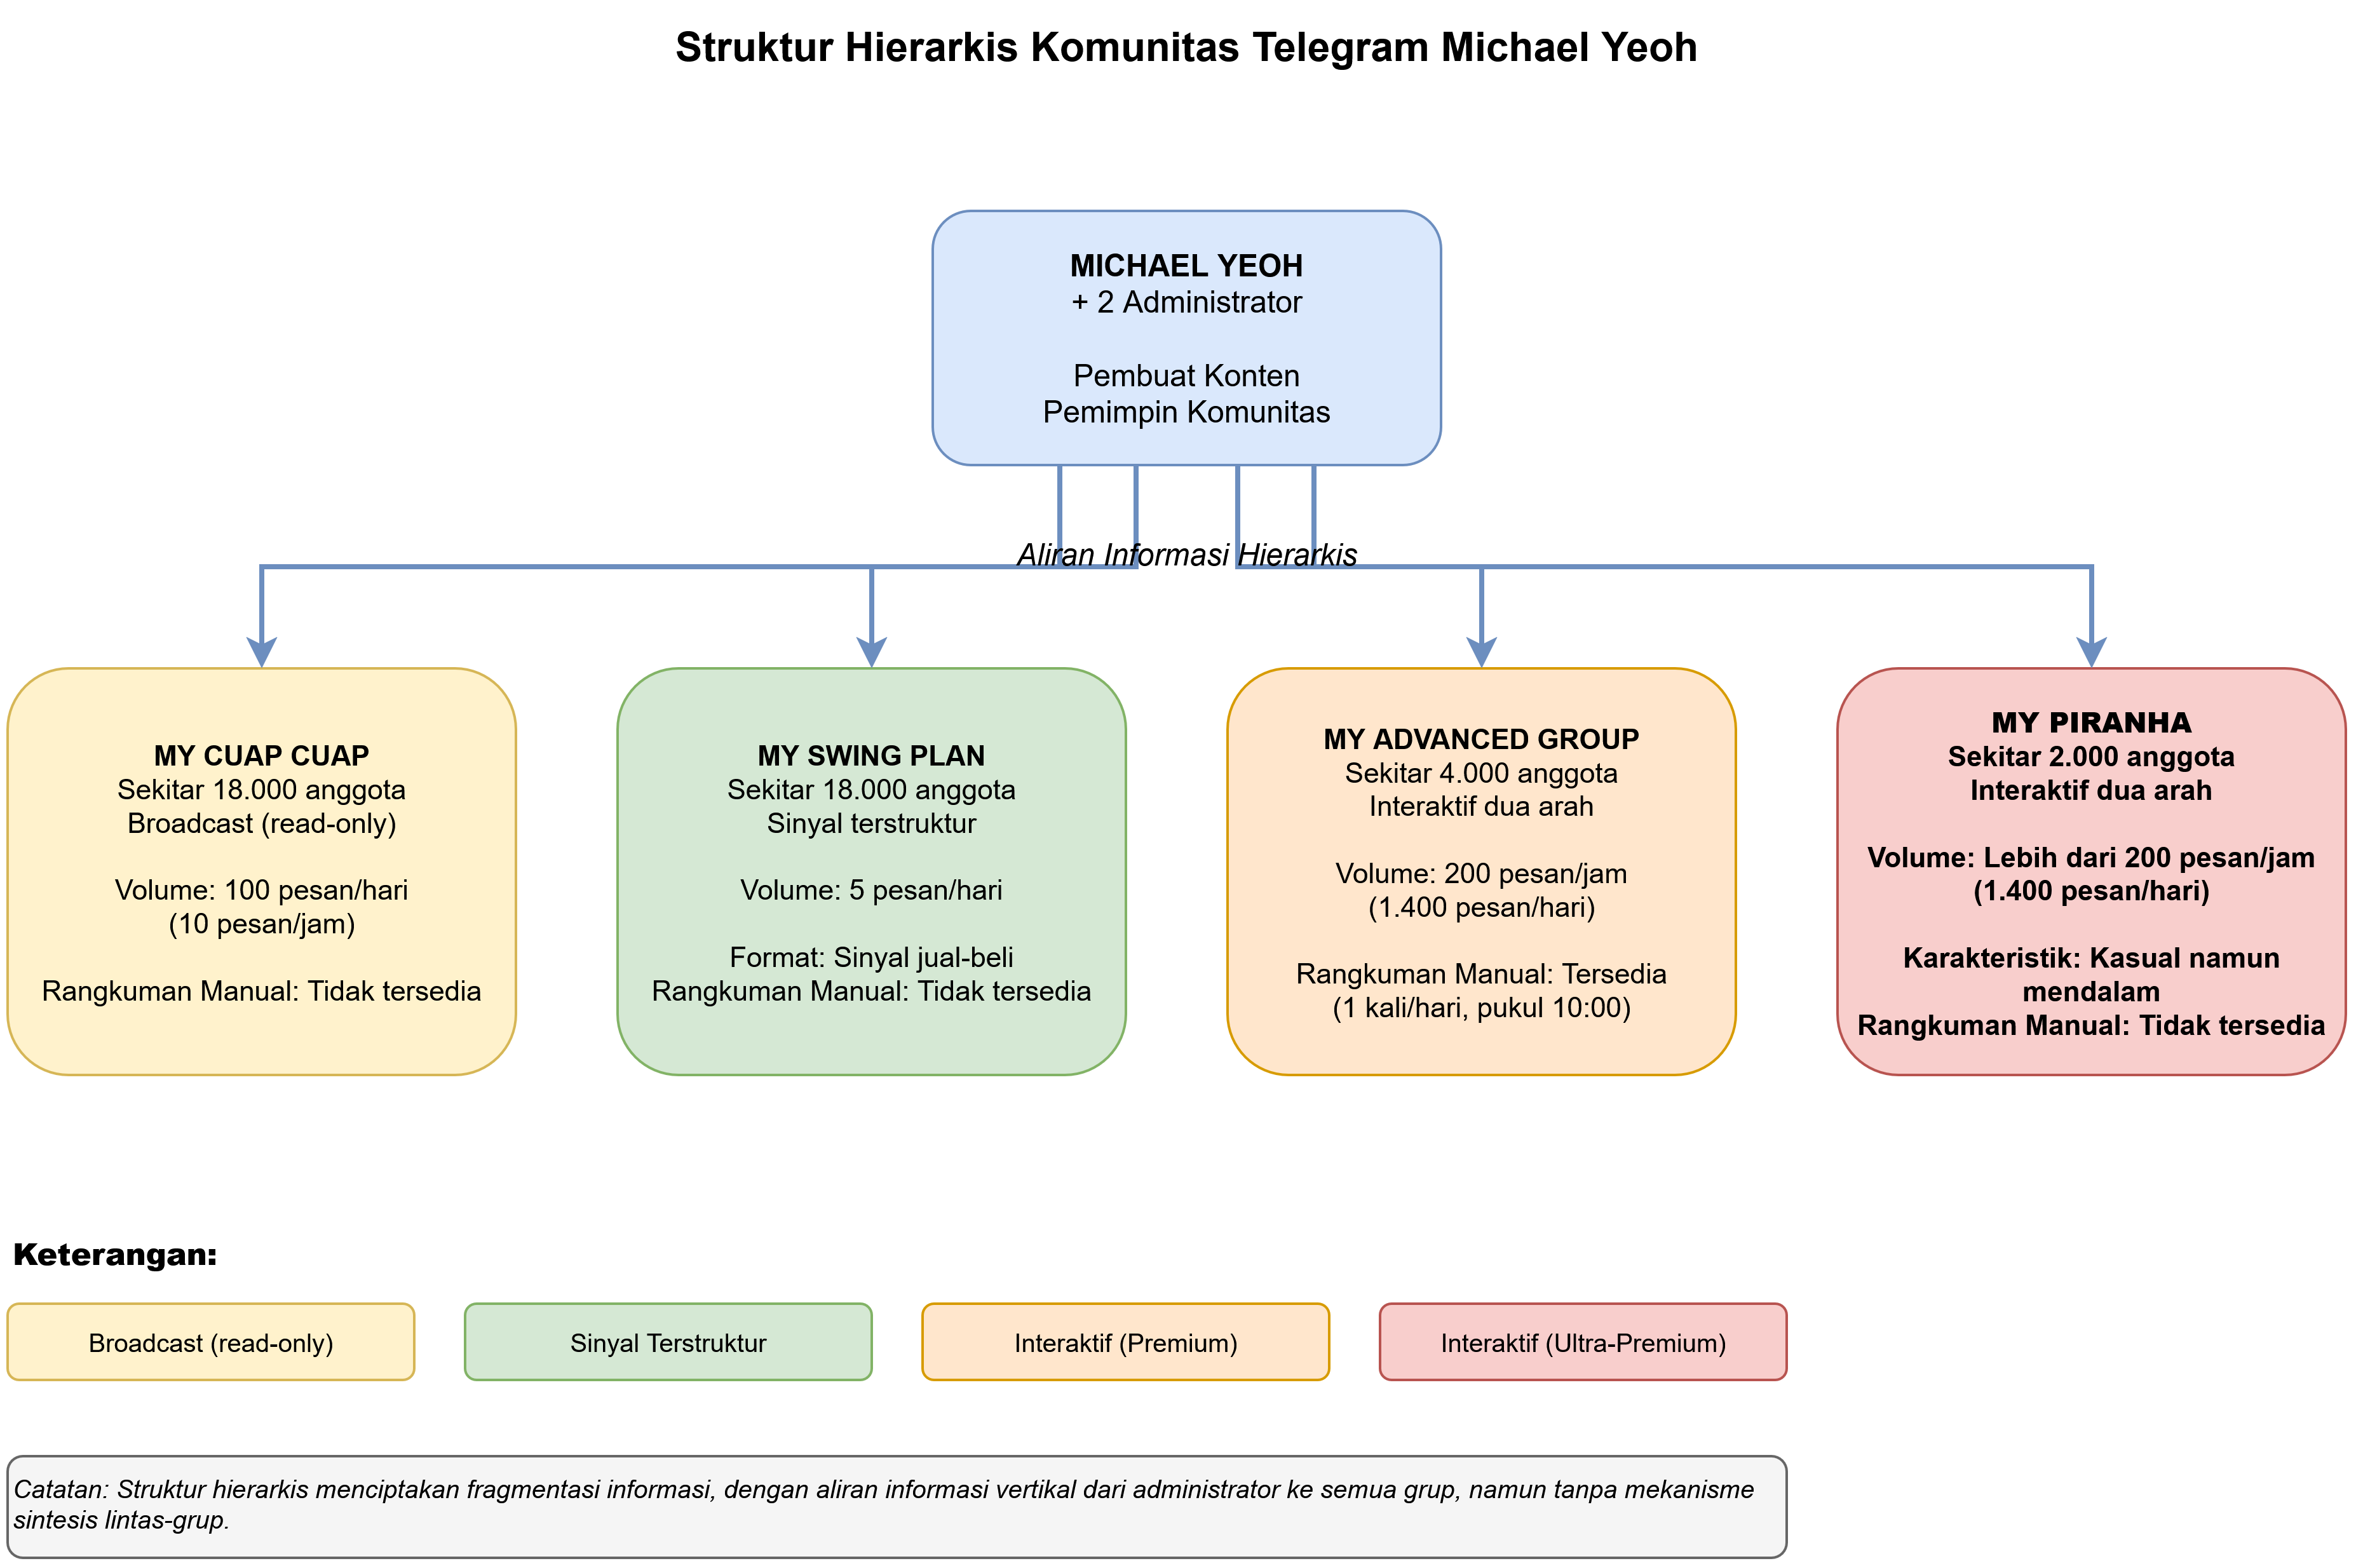
\includegraphics[width=0.9\textwidth]{image/current-state-diagram.png}
  \caption{Model konseptual sistem komunikasi komunitas Telegram Michael Yeoh}
  \label{fig:current-system}
\end{figure}

Struktur hierarkis komunitas dapat dilihat secara komprehensif pada Tabel \ref{tab:group-characteristics}.\footnote{Data jumlah anggota berdasarkan kondisi per 4 November 2025. Jumlah anggota bersifat dinamis dan terus bertambah seiring pertumbuhan komunitas.} Setiap grup memiliki fungsi spesifik dalam ekosistem informasi, dengan kompleksitas komunikasi yang meningkat seiring level hierarki.

\begin{longtable}{@{\extracolsep{\fill}} p{3cm} p{2.5cm} p{2.5cm} p{3cm} p{2.5cm}}
\caption{Karakteristik grup dalam komunitas Telegram Michael Yeoh (per 4 November 2025)}
\label{tab:group-characteristics} \\
\toprule
\textbf{Aspek} & \textbf{Cuap Cuap} & \textbf{Swing Plan} & \textbf{Advanced} & \textbf{PIRANHA} \\
\midrule
\endfirsthead

\caption{Karakteristik grup dalam komunitas Telegram Michael Yeoh (lanjutan)} \\
\toprule
\textbf{Aspek} & \textbf{Cuap Cuap} & \textbf{Swing Plan} & \textbf{Advanced} & \textbf{PIRANHA} \\
\midrule
\endhead

\midrule
\multicolumn{5}{r}{\textit{Bersambung ke halaman berikutnya}} \\
\bottomrule
\endfoot

\bottomrule
\endlastfoot

Jumlah Anggota & 20.500 & 20.500 & 4.300 & 2.000 \\
Tipe Komunikasi & \textit{Broadcast} (\textit{read-only}) & Sinyal terstruktur & Interaktif dua arah & Interaktif dua arah \\
Volume Pesan & 100 pesan per hari (10 per jam) & 5 pesan per hari & 200 pesan per jam & Lebih dari 200 pesan per jam \\
Konten Utama & Edukasi umum dan berita pasar & Sinyal jual-beli terstruktur & Diskusi analisis teknikal & Debat strategi investasi \\
Rangkuman Manual & Tidak tersedia & Tidak tersedia & Tersedia (1 kali per hari, pukul 10:00) & Tidak tersedia \\
Tingkat Masalah & Rendah & Minimal & Tinggi & Sangat Tinggi \\
\end{longtable}

Grup MY Cuap Cuap dan MY Swing Plan berfungsi sebagai kanal informasi dengan mode \textit{read-only} atau sinyal terstruktur. MY Cuap Cuap menyediakan edukasi pasar dan analisis makroekonomi dengan volume 100 pesan per hari, sementara MY Swing Plan mendistribusikan sinyal \textit{trading} terstruktur (contoh: "BGTG BUY 106-100 SL 98 porsi 5\%") dengan volume hanya 5 pesan per hari. Kedua grup ini memiliki tingkat \textit{information overload} rendah namun menjadi bagian penting dari ekosistem yang memerlukan sintesis dengan diskusi di grup premium.

Grup MY Advanced Group merupakan grup premium pertama dengan komunikasi interaktif dua arah untuk 4.300 anggota. Volume pesan mencapai 200 pesan per jam selama jam perdagangan (09:00-16:00), menghasilkan sekitar 1.400 pesan per hari. Grup ini memiliki satu rangkuman manual oleh asisten Richy Matthew Ashari setiap pukul 10:00, namun hanya mencakup jam pertama perdagangan (09:00-10:00), meninggalkan gap enam jam berikutnya.

Grup MY PIRANHA, sebagai grup ultra-premium dengan 2.000 anggota elite, mengalami volume pesan tertinggi (lebih dari 200 pesan per jam) namun tanpa rangkuman manual sama sekali. Diskusi cenderung kasual dalam gaya namun sangat mendalam secara konten, menciptakan tantangan ekstraksi sinyal karena informasi penting sering tersembunyi dalam percakapan informal tanpa penanda eksplisit.

Aliran informasi bersifat hierarkis dengan fragmentasi sistemik. Michael Yeoh dan administrator dapat memposting di semua grup, menciptakan aliran vertikal dari puncak hierarki. Namun, anggota di level berbeda tidak dapat mengakses grup yang lebih tinggi, menciptakan fragmentasi informasi antara analisis makro (Cuap Cuap), sinyal konkret (Swing Plan), diskusi implementasi (Advanced), dan debat strategi (PIRANHA). Anggota yang mengikuti multiple grup harus melakukan sintesis manual lintas grup, yang memerlukan waktu dan kemampuan analisis signifikan.

\subsection{Implikasi untuk Desain Sistem Rangkuman Otomatis}

Karakteristik unik komunitas ini—volume pesan ekstrim, struktur hierarkis eksplisit, konten domain finansial Indonesia, dan penggunaan Bahasa Indonesia informal—menjadikannya kasus yang ideal untuk pengembangan dan evaluasi sistem rangkuman otomatis berbasis \textit{AI} yang dioptimalkan untuk konteks lokal. Sistem yang dikembangkan dalam penelitian ini dirancang untuk mereduksi beban informasi melalui rangkuman periodik yang mensintesis intelijen lintas-grup, dengan memanfaatkan literatur tentang \textit{information overload}, \textit{cognitive load theory}, NLP finansial, dan infrastruktur sistem \textit{real-time} yang telah diulas dalam bab ini.

Analisis mendalam terhadap identifikasi masalah spesifik, kebutuhan sistem, dan alternatif solusi akan diuraikan secara komprehensif dalam Bab \ref{chap:analisis-masalah}.